\documentclass{article}
\usepackage[utf8]{inputenc}

\title{Laboratorio01U2_INTELIGENCIA_NEGOCIOS}
\author{edwartbalcon}
\date{Septiembre 2021}

\usepackage[utf8]{inputenc}
\usepackage[spanish]{babel}
\usepackage{natbib}
\usepackage{graphicx}

\begin{document}

\title{Caratula}

\begin{titlepage}
\begin{center}
\begin{Large}
\textbf{UNIVERSIDAD PRIVADA DE TACNA} \\
\end{Large}
\vspace*{-0.025in}
\begin{figure}[htb]
\begin{center}

\includegraphics[width=6cm]{./images/logo_UPT}
\end{center}
\end{figure}
\vspace*{-0.025in}
\begin{Large}
\textbf{FACULTAD DE INGENIERIA} \\
\end{Large}
\vspace*{0.05in}
\begin{Large}
\textbf{Escuela Profesional de Ingeniería de Sistema} \\
\end{Large}


\vspace*{0.4in}

\vspace*{0.1in}
\begin{Large}
\textbf{Informe de laboratorio 02: Importación, Data FloW, traslado de archivos} \\
\end{Large}

\vspace*{0.3in}
\begin{Large}
\textbf{Curso: Inteligencia de negocios} \\
\end{Large}

\vspace*{0.3in}
\begin{Large}
\textbf{DOCENTE: Ing. Patrick Cuadros Quiroga} \\
\end{Large}

\vspace*{0.2in}
\vspace*{0.1in}
\begin{large}

\begin{Large}
\textbf{Alumno: Balcon Coahila, Edwart Juan\hfill	(2013046516) } \\
\end{Large}

\vspace*{0.15in}
\begin{Large}
\textbf{Tacna – Perú} \\
\end{Large}

\vspace*{0.05in}
\begin{Large}
\textbf{2021 } \\
\end{Large}

\end{large}
\end{center}

\end{titlepage}


%% ----------------------------------------------------------------------------------------------------------------------------------
\begin{center}
\begin{LARGE}
	\textbf{Práctica de Laboratorio N° 02: \\ Importación, Data Flow y Traslado de Archivos} \\ 
\end{LARGE}
\rule{175mm}{0.1mm}
\end{center}



%% ----------------------------------------------------------------------------------------------------------------------------------

\section{Objetivos}

\begin{itemize}
\item Importar datos usando el WIZARD 
\item Desarrollar mis primeros Paquetes DTSX

\end{itemize}

%% ----------------------------------------------------------------------------------------------------------------------------------
\section {\textbf{Requerimientos}}

\subsection{\textbf{Conocimientos}}
Para el desarrollo de esta práctica se requerirá de los siguientes conocimientos básicos:
\begin{itemize}
\item Conocimientos básicos de administración de base de datos Microsoft SQL Server.
\item Conocimientos básicos de SQL.
\end{itemize}



\subsection{\textbf{Software}}
Asimismo se necesita los siguientes aplicativos:
\begin{itemize}
\item SQL Server Integration Services
\item BD Adventure Work (OLTP y Data Warehouse)
\item BD AdventureWorkLT2012
\end{itemize}


	\begin{figure}[htb]
		\begin{center}
			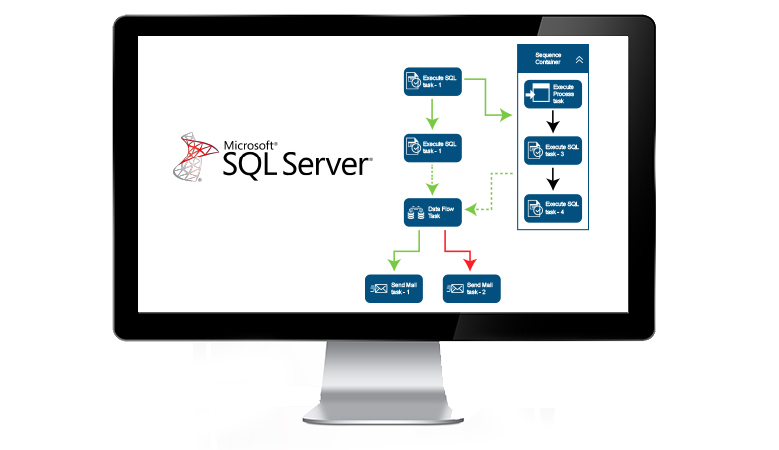
\includegraphics[width=13cm]{./images/MS-SQL-Server-Integration-Services}
			
		\end{center}
	\end{figure}



%% ----------------------------------------------------------------------------------------------------------------------------------
\newpage

\section{Desarrollo}

%% TAREA 1-------------------------------------------------------------------------------------------------------------------

\subsection{TAREA N° 01: Importación de datos usando el WIZARD – SQL Managment}

\begin{itemize}
\item Crear una base de datos – BDTEST
	\begin{figure}[htb]
		\begin{center}
			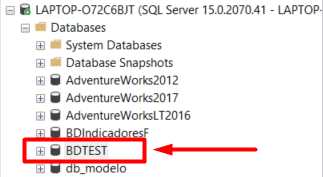
\includegraphics[width=8cm]{./images/Tarea1_1}
			
		\end{center}
	\end{figure}
\item Importar Datos desde AdventureWorks
	\begin{figure}[htb]
		\begin{center}
			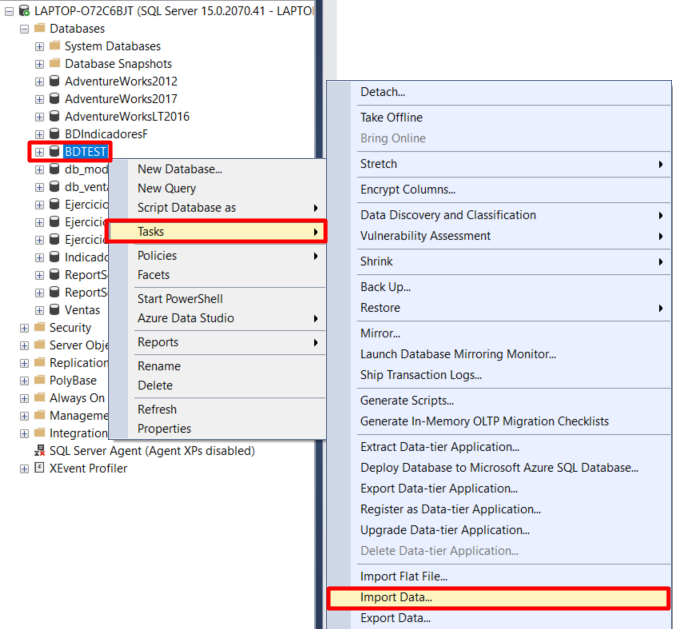
\includegraphics[width=13cm]{./images/Tarea1_2}
			
		\end{center}
	\end{figure}

\newpage

\item Next y escribir el Servidor y seleccionar la base de datos
\item \textbf{Data Source:} La base de donde vamos a importar
\item \textbf{Destination:} La Base donde vamos a cargar la data
	\begin{figure}[htb]
		\begin{center}
			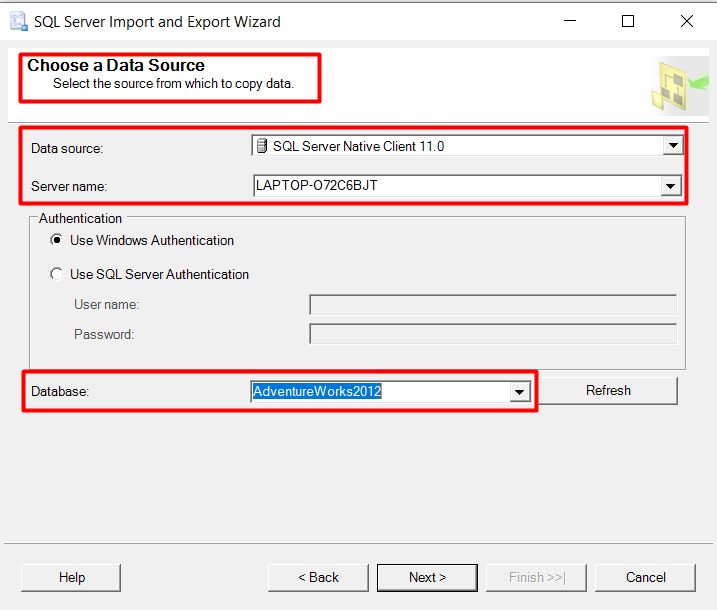
\includegraphics[width=8cm]{./images/Tarea1_3}
			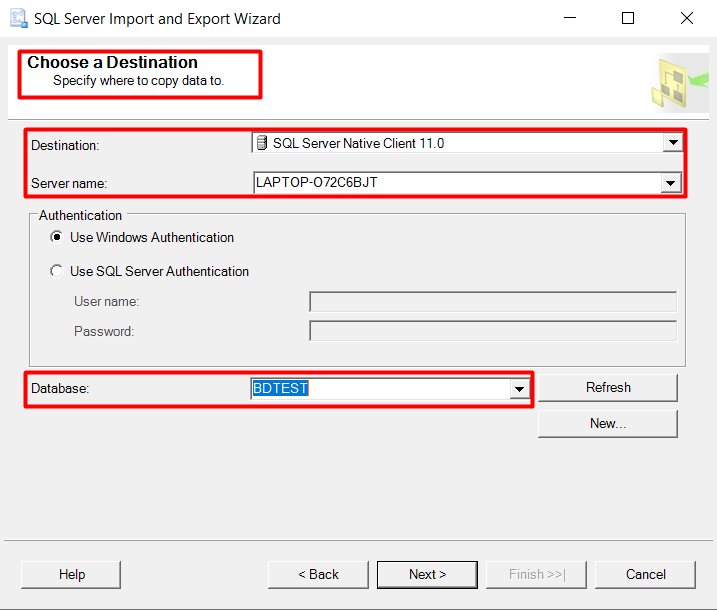
\includegraphics[width=8cm]{./images/Tarea1_4}
		\end{center}
	\end{figure}

\item Podemos copiar los datos desde una o mas tablas o vistas. 
\item También podemos recuperar datos mediante una consulta SQL.
\item Seleccionamos: HumanResources.Department y Person.Address
	\begin{figure}[htb]
		\begin{center}
			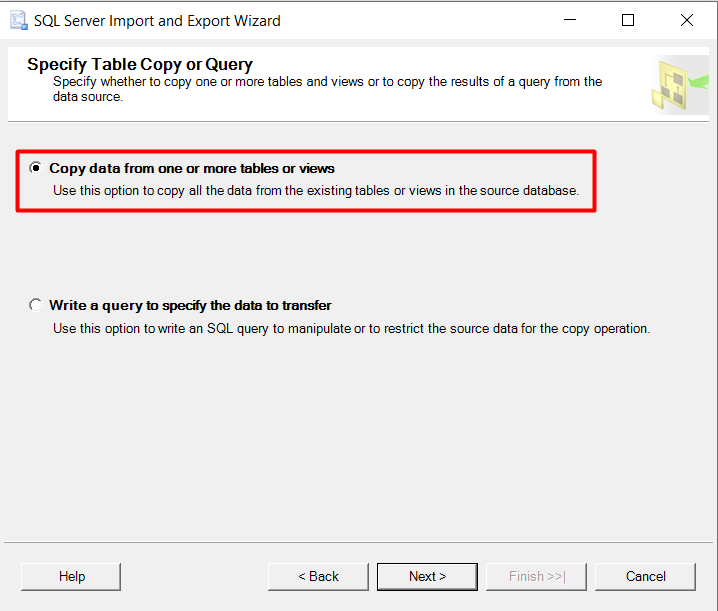
\includegraphics[width=8cm]{./images/Tarea1_5}
			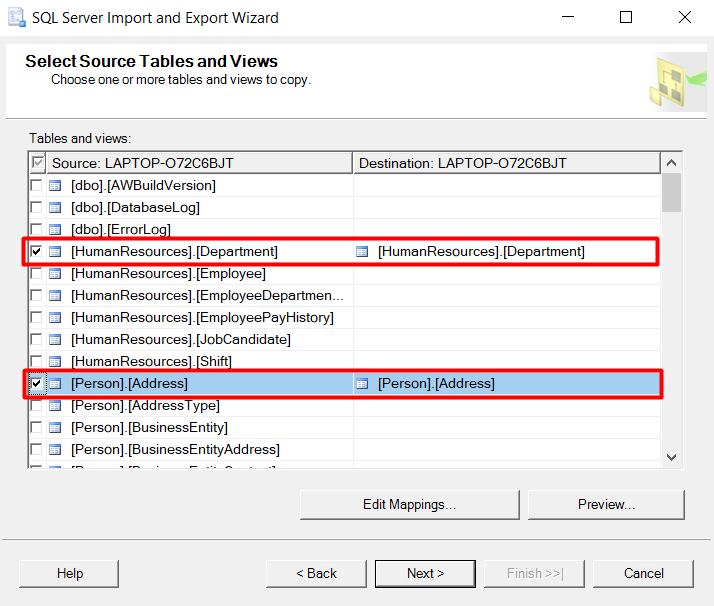
\includegraphics[width=8cm]{./images/Tarea1_6}
		\end{center}
	\end{figure}

\newpage

\item Activamos para guardar el paquete.
\item Indicamos el lugar donde que va a guardar el DTSX.
	\begin{figure}[htb]
		\begin{center}
			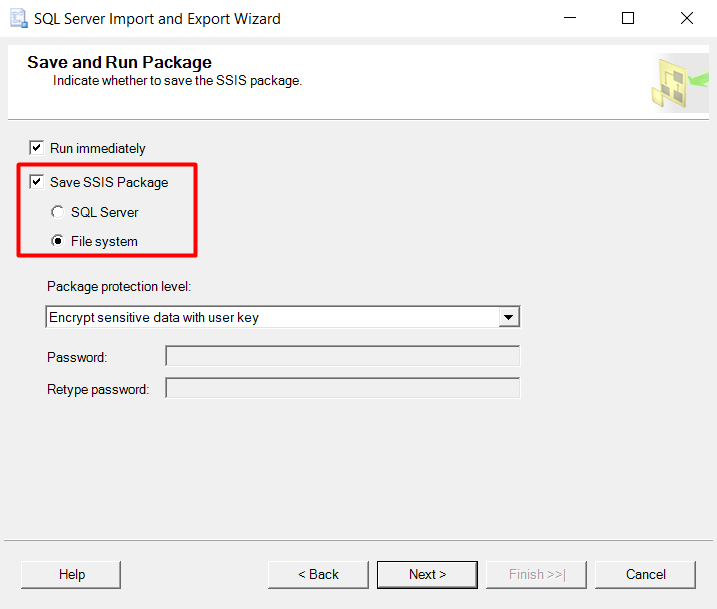
\includegraphics[width=8cm]{./images/Tarea1_7}
			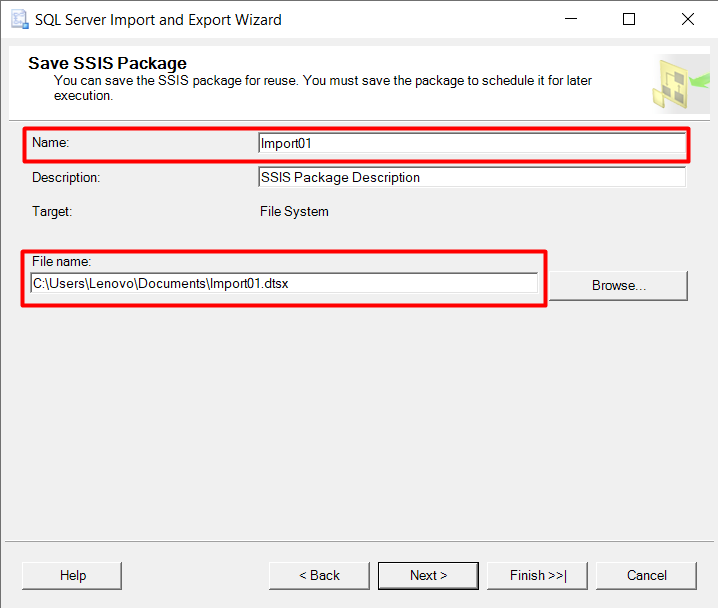
\includegraphics[width=8cm]{./images/Tarea1_8}
		\end{center}
	\end{figure}



\item Le damos clic a Finalizar para completar las acciones.
\item Al finalizar tenemos el resumen de la ejecución
\item Hemos generado nuestro primer paquete de forma automática.
	\begin{figure}[htb]
		\begin{center}
			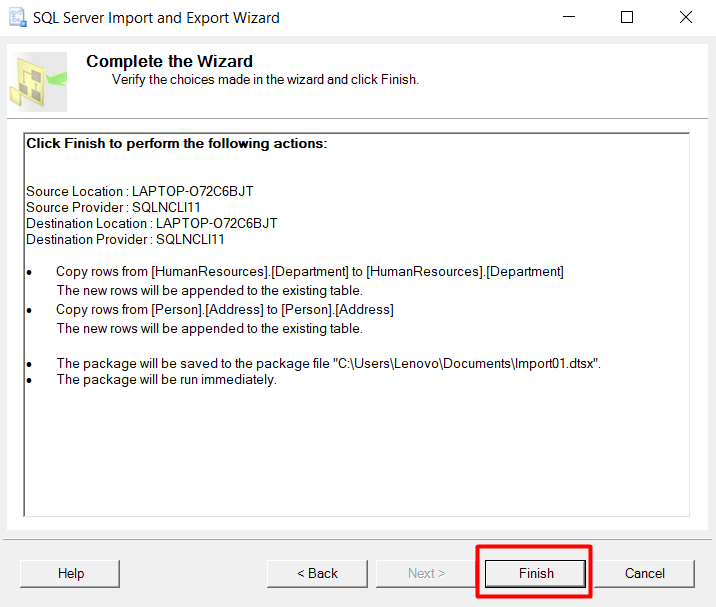
\includegraphics[width=8cm]{./images/Tarea1_9}
			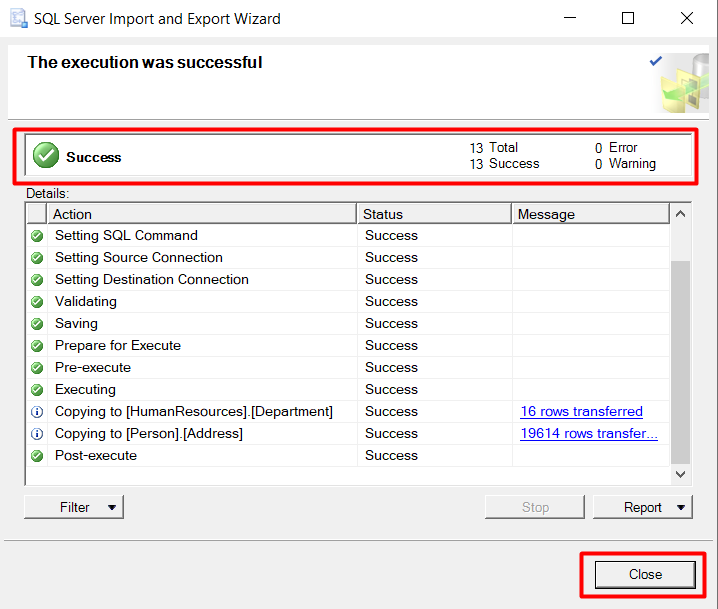
\includegraphics[width=8cm]{./images/Tarea1_10}
		\end{center}
	\end{figure}

\newpage

\item Podemos actualizar la Base de Datos BDTEST y encontraremos las tablas ya importadas
	\begin{figure}[htb]
		\begin{center}
			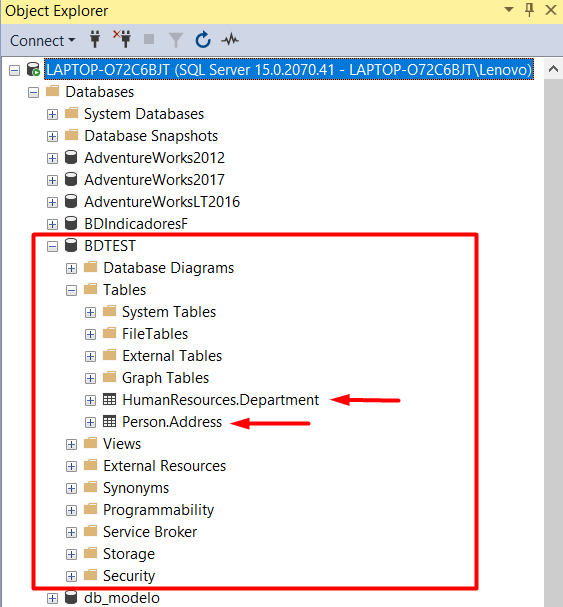
\includegraphics[width=12cm]{./images/Tarea1_11}
		\end{center}
	\end{figure}

\end{itemize}

\newpage

%% TAREA 2-------------------------------------------------------------------------------------------------------------------

\subsection{TAREA N° 02: Creamos nuestro primer Paquete DTSX}

\begin{itemize}
\item Crear una base de datos – BDTEST
	\begin{figure}[htb]
		\begin{center}
			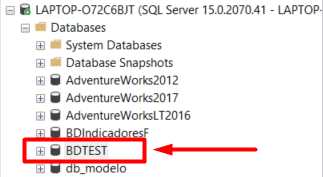
\includegraphics[width=8cm]{./images/Tarea1_1}
			
		\end{center}
	\end{figure}
\item Importar Datos desde AdventureWorks
	\begin{figure}[htb]
		\begin{center}
			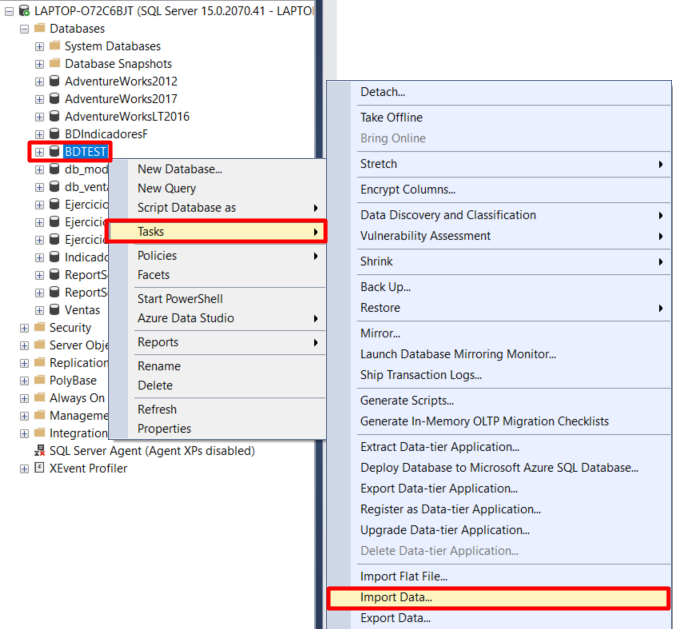
\includegraphics[width=13cm]{./images/Tarea1_2}
			
		\end{center}
	\end{figure}

\newpage



\end{itemize}



\end{document}
